\section{Az EGTIB bemutatása}
\begin{frame}
	\frametitle{Az EGTIB bemutatása}
	\begin{block}{Az EGTIB projekt célja}
		\begin{itemize}
			\item felhasználóbarát felület
			\item lehetőség a daganatos sejtek modellezésére 
			\item és szimulációjára
			\pause
			\item a szimulációs eredmények megjelenítésére
		\end{itemize}
	\end{block}

	\begin{figure}[ht!]
		\centering
		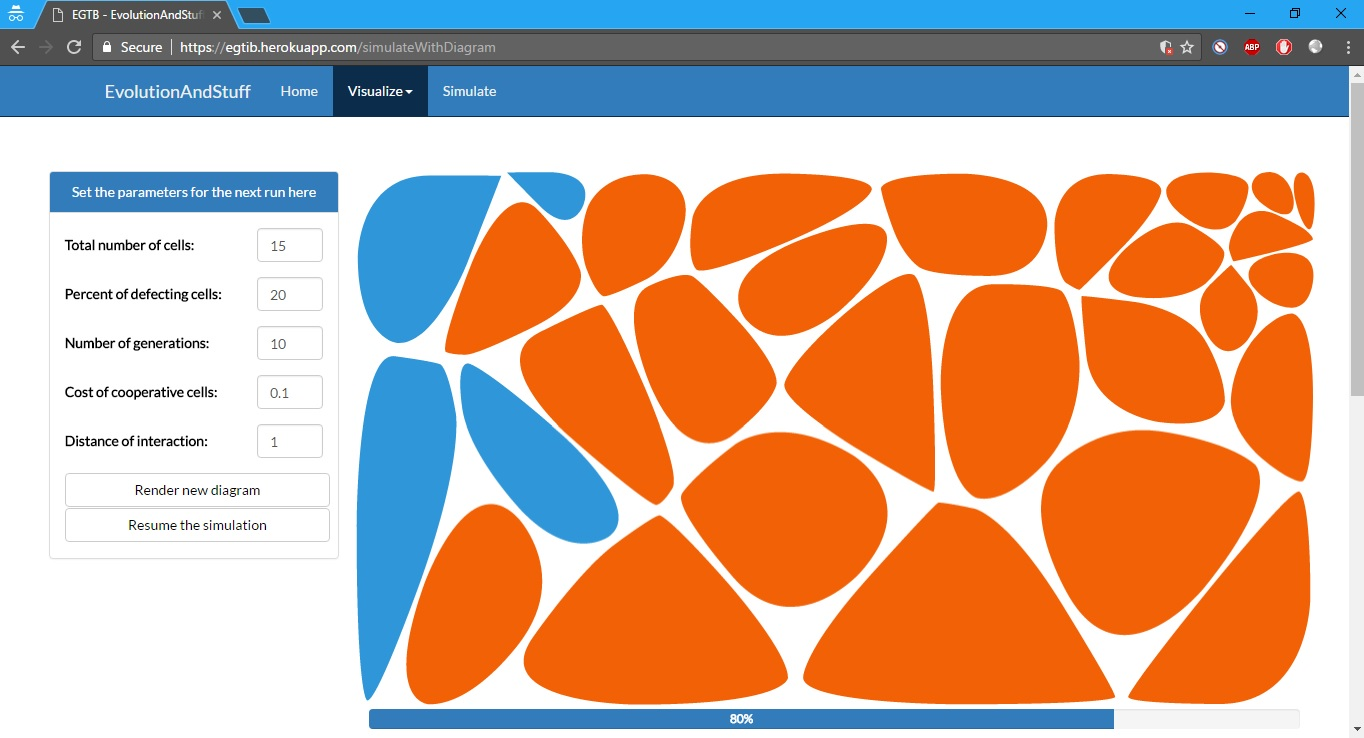
\includegraphics[width=0.6\linewidth]{images/EGTIB.jpg}
		\caption{Pillanatkép az alkalmazásról}
		\label{fig:SimulateWithDiagram}
	\end{figure}
\end{frame}

\subsection{Funkcionalitások}
\begin{frame}
	\frametitle{Funkcionalitások}
	\begin{block}{Válaszható paraméterek}
		\begin{itemize}
			\item kezdeti populáció mérete
			\item defektálók aránya 
			\item generáció szám (szimuláció hossza)
			\item kooperáló sejtek termelési költsége 
			\item diffúziós távolság mérete
			\item legyenek a sejtek osztódásra képesek?
		\end{itemize}
	\end{block}
\end{frame}

\begin{frame}
	\frametitle{Demó}
	\Huge{\centerline{Demó}}
\end{frame}

\subsection{Felhasznált technológiák}
\begin{frame}
\frametitle{Felhasznált technológiák}
\begin{figure}[ht!]
	\centering
	
\includegraphics[width=\linewidth]{images/technologies}
\end{figure}
\end{frame}
